%!TEX root = ../thesis.tex
\chapter{Background}
\label{ch:background}

This thesis uses newly developed approaches from applied topology to study problems in evolutionary biology and genomics.
Here we supply sufficient background to motivate our approach.

\section{Biology}

In this section we present a basic introduction to molecular sequence data: what the data looks like, the processes by which it is generated, and the methods by which it is analyzed.
Particular attention is paid to modes of reticulate evolution.
Exposition for specific applications can be found in their respective individual chapters.

\subsection{Genes and Genomes}

The information required to express an organism's biological form and function is contained in the genome.
Physically, the genome is manifest as a sequence of nucleotides (DNA), at least one copy of which is packaged inside each cell of an organism.
Abstractly, the genome is represented as a linear sequence of characters defined over the alphabet $\{A,C,G,T\}$.\footnote{The linear representation can be misleading, as many organisms, primarily viruses and bacteria, have circular genomes.}
Contained in this sequence are subsequences representing genes, which code for the protein products that ultimately affect function.
Further embedded in the genome is a complex regulatory pattern of transcription factors controlling the expression of particular genes and directing cellular differentiation and development.

Following the central dogma of biology, DNA is transcribed into RNA, RNA is translated into amino acids, and amino acids are folded into proteins \cite{Crick:1970wb}.
Proteins comprise the functional unit of biology.

Beyond simply coding for function, the genome includes an imprint of the evolutionary history that gave rise to the organism.
By comparing the genomes of multiple organisms, inferences can be drawn about the evolutionary relationships among extant organisms as well as the processes that generated bserved diversity.
The field concerned with exploring these relationships is \emph{comparative genomics}.

\subsection{Evolutionary Processes}

Evolution describes the gradual change in phenotypes arising from random variation and subject to natural selection.
The processes giving rise to diversity can be classified into two types: clonal and reticulate.

\subsubsection{Clonal Evolution}

Clonal evolution, or vertical evolution, is a process of self-reproduction whereby genetic material is transferred directly from parent to offspring.
Population diversity is generated by stochastic mutation and maintained over multiple generations by random drift.

It is clonal evolution that Darwin had in mind when he described the idea of descent with modification, whereby a parent passes genomic information to an offspring subject to random drift.
Importantly, because there is always a direct parent--offspring relationship, clonal evolution will be consistent with a phylogenetic tree model.

\subsubsection{Reticulate Evolution}

Reticulate evolution, or horizontal evolution, refers to exchange or acquisition of genetic material via processes that do not reflect a direct parent--offspring relationship.
As we will see, these processes can make inferences about historical evolutionary relationships difficult.
Different types reticulate processes occur in different types of organisms (summarized in Table \ref{table:reticulation_processes}).

Viruses replicate by infecting a host cell and then using the host cell machinery and resources to produce multiple copies of viral genetic material.
The genetic material is then packaged into new virus particles which are shed off in order to infect new cells.
Reticulation can occur when two virus particles coinfect the same host cell.
During the replication process, genetic material can be exchanged in one of two ways: \emph{reassortment} or \emph{recombination} (the two processes are contrased in Figure~\ref{fig:viral_reticulation}).
Reassortment occurs in viruses whose genomes are segmented, such as influenza.
Segments are similar to chromosomes, such that a single virus particle will contain a single copy of each segment.
Reassortment occurs when coinfection results in packaging of segments taken from different virus particles.
The result viral progeny will then be a genetic mixture of segments from each parental strain.
Recombination, more common in nonsegmented viruses such as HIV, involves a break-rejoin mechanism during the replication process.
Here, an error in the polymerase during replication can result in an incomplete copy of the genome (a break).
At this point, several cellular processes involved in repair can be recruited to complete the replication process using a homologous region.
If coinfection has occurred, it is possible for these processes to initiate repair using material from a different parental strain.
The outcome will be novel genetic material that includes a crossover from one strain to another.
Break-rejoin crossover is a type of \emph{homologous recombination}.

\begin{figure}
\centering
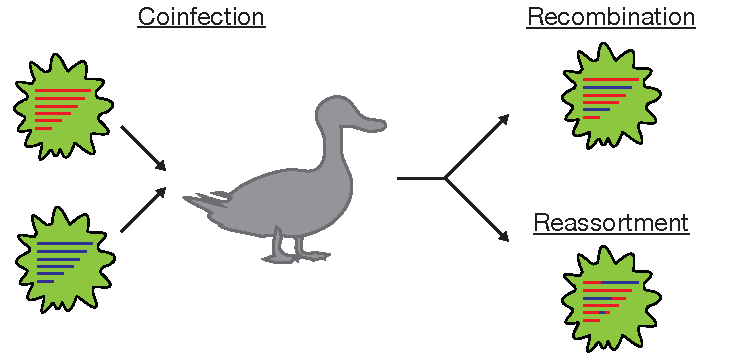
\includegraphics[]{./fig/background/viral_reticulation.pdf}
\caption[Viral recombination and reassortment]{The two modes of viral reticulation. Coinfection of the same host cell can lead to either reassortment, in which whole viral segments are exchanged, or recombination, in which breakpoints can occur within segments. The former process is common in influenza, the latter in HIV. The end result, however, is a novel virus particle which shares genetic information from both parents.}
\label{fig:viral_reticulation}
\end{figure}

In bacteria and other prokaryotes, reticulate evolution can occur when foreign DNA from a donor is acquired by a target organism and integrated into its genome.
Three generic mechanisms have been identified, depending on the route by which foreign DNA is acquired \cite{Ochman:2000dr}:
\begin{enumerate}
\item \emph{Conjugation}. Direct cell-to-cell contact between donor and recipient resulting in transfer of plasmid.
\item \emph{Transformation}. Foreign DNA acquired via uptake from freely circulating DNA in the environment.
\item \emph{Transduction}. Virus-mediated transfer for foreign DNA from an infected donor cell.
\end{enumerate}
A visualization of these three mechanisms is shown in Figure~\ref{fig:bacterial_reticulation}.
Beause these mechanisms can often lead to the acqusition of novel sequences coding for genes not in the recipient organism, reticulate evolution in prokaryotes is often called \emph{horizontal gene transfer} or \emph{lateral gene transfer}.

\begin{figure}
\centering
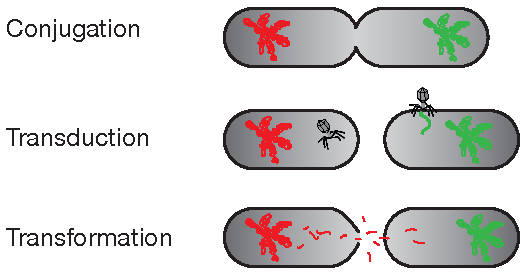
\includegraphics[]{./fig/background/bacterial_reticulation.pdf}
\caption[Three modes of bacterial reticulation]{Three modes of viral reticulation. (1) Conjugation, in which direct cell-to-cell contact results in transfer of genetic material; (2) Transformation, in which foreign DNA is acquired via uptake from freely circulating DNA in the environment; and (3) Transduction, in which exchange of genetic material is mediated by a virus or phage particle.}
\label{fig:bacterial_reticulation}
\end{figure}

In eukaryotes, several reticulate processes have been identified.
We mention two such processes: hybrid speciation and meitotic recombination.
These two processes act at very different scales, but the outcome is the same: a distinct offspring with genetic material 

First, hybrid speciation refers to the cross-breeding of animals or plants of different species.
This mixing of genetic material can lead to the development of a third species with a phenotype distinct from both parents.
Hybrid speciation was originally believed to be a rare occurrence in nature and hybrid offspring to be infertile.
However, recent genomic data has demonstrated that hybrid speciation occurs quite frequently in plants \cite{Arnold:1996,Arnold:2007vq}.
Indeed, Mendel's early experiments in hybridization were themselves an artifically induced form of reticulate evolution.

Second, meiotic recombination refers to a specialized process for generating diversity that occurs in sexually-reproducing polyploid organisms, such as humans, during meiosis.
Meiosis is the process by which a single cell containing $n$ copies of each chromosome results in four distinct cells each with $n/2$ copies of each chromosome.
These special cells are called gametes.
Sexual reproduction consists of the fusion of two gametes during fertilization to form a zygote, which ultimately develops into a viable offspring.
Meiosis is a multistep process consisting of an initial round of DNA replication followed by two rounds of cell division.
Meiotic recombination occurs after the initial round of DNA replication and prior to cell division.
After DNA replication, there are two copies of each homologous chromosome that are joined at a centromere.
The two sets of chromosomes then pair with each other and exchange DNA through physical interactions known as crossovers.\footnote{These crossovers have been shown to not occur randomly, but rather at recombination hotspots regulated by binding motifs for by the PRDM9 protein. \kje{Cite Pablo Paper and a Molly paper}.}
This is another example of homologous recombination and results in new allelic patterns mixing genetic information from both parents.\footnote{Patterns of shared alleles define the concept of \emph{linkage}.}
After crossover occurs, two phases of cellular division result in gametes with $n/2$ copies of each chromosome.

At this junction, one might wonder about sexual reproduction -- an offspring can be seen as a hybridization of genetic material from both mother and father.
Is sex then a form of reticulate evolution?
On the one hand, the answer could be yes, particularly because the presence of meiotic recombination involves a shuffling of genomic material such that the chromosome each parent donates is a unique combination of sequence not previously present.
On the other hand, the answer could be no, because both mother and father donate a complete copy of the genome to the offspring.
Each copy can be considered an independent transfer and defined to be a pattern
On the other hand, the answer could be no, because each mother and father donates an entire copy of the genome to the offspring.
Each copy can be considered an independent transfer.
Indeed, researchers in human population genetics generally disintinguish between the most common ancestor on the patrilineal line and the matrilineal line.
On the other


In fact, reproduction of $n$-ploid organisms is often analyzed mathematically as the 


One might wonder about sexual reproduc

\footnote{One might wonder about sexual reproduction -- a descendent can be seen as a hybridization of both mother and father. Indeed, sexual reproduction can itself be considered a form of reticulate evolution. In the case of \emph{H. sapiens}, a diploid species with two copies of each chromosome, XXX. However, from an evolutionary perspective, the process can be decoupled into two independent clonal processes. When discussing the human species, researchers will commonly refer to the most recent common ancestor on the patrilineal as Y-chromosomal Adam and the most recent common ancestor on the matrilineal as mitochondrial Eve.}

\begin{tabularx}{\textwidth}{lll}
\toprule
Organism & Process & Description \\
\midrule
\multirow{2}{*}{Virus} & Reassortment & INSERT FIGURE \\
                       & Recombination & INSERT FIGURE \\
\midrule
\multirow{3}{*}{Bacteria} & Transformation & xx \\
                          & Transduction   & xx \\
                          & Conjugation    & xx \\
\midrule
\multirow{2}{*}{Eukaryotes} & Meiotic Recombination & Description \\
                            & Hybrid Speciation         & Description \\
\bottomrule
\label{table:reticulation_processes}
\end{tabularx}

The presence of horizontal gene transfer in a set of organisms can be most clearly identified by comparing the phylogenetic trees built from different genes.
If horizontal gene transfer has occurred, the set of \emph{gene trees} will reflect different evolutionary relationships and not be consistent with a single tree topology.
A subfield of comparative genomics is concerned with building \emph{species trees} from sets of gene trees, however in the case where there is substantial disagreement among gene trees the very notion of a species tree may be flawed.

Traditionally, evolutionary biology has concerned itself with characterizing relationships in light of vertical evolution alone.
However, increasing evidence \kje{(what evidence?)} has pointed to the important role played by horizontal evolution, particularly in prokaryotic evolution.
\kje{[Further citations and exposition of Doolittle, Koonin, and Gogarten.]}

\subsection{Mathematical Models of Evolution}

Mathematical population genetics is concerned with properties of populations as they are subject to evolutionary forces over long time scales.
These forces include natural selection, genetic drift, mutation, and recombination.
Historically the input data for population genetics models was comparative studies of allele frequencies across populations.
These studies have primarily been replaced by large-scale genomic surveys which have provided unprecedented insight into ancient population structure and historical migrations.
\kje{[Give an example and cite work of reich / bustamente, etc.]}

Incorporate understanding of real data
These models allow two things: 1) simulate genomic data under realistic processes and 2) build statistical models to estimate biological parameters from real data.

\subsubsection{The Wright-Fisher Model}

The Wright-Fischer model is a forward time simulation of an evolving population.
In the simplest case, the model describes neutral evolution of a constant population size with no structure and constant genome length.
The model proceeds in units of generations.
At each generation, a member of the population is an offspring of a randomly selected ancestor from the previous generation.
This offspring inherits its ancestors genomes, with mutations introduced at some base rate $\mu$.
A member of previous generation with no offspring will be considered extinct.
\kje{[Figure comparing Wright-Fisher and Coalescent.]}

\subsubsection{The Coalescent Process}

The coalescent process is a stochastic model that generates the genealogy of individuals sampled from an evolving population \cite{Wakeley:2009}.
The genealogy is then used to simulate the genetic sequences of the sample.
This model is essential to many methods commonly used in population genetics.
Starting with a present-day sample of $n$ individuals, each individual's lineage is traced backward in time, towards a mutual common ancestor.
Two separate lineages collapse via a coalescence event, representing the sharing of an ancestor by the two lineages.
The stochastic process ends when all lineages of all sampled individuals collapse into a single common ancestor.
In this process, if the total (diploid) population size $N$ is sufficiently large, then the expected time before a coalescence event, in units of $2N$ generations, is approximately exponentially distributed:
\begin{equation}
P(T_{k}=t) \approx \binom{k}{2} e^{-\binom{k}{2} t},
\end{equation}
where $T_k$ is the time that it takes for $k$ individual lineages to collapse into $k-1$ lineages.

After generating a genealogy, the genetic sequences of the sample can be simulated by placing mutations on the individual branches of the lineage.
The number of mutations on each branch is Poisson-distributed with mean $\theta t / 2$, where $t$ is the branch length and $\theta$ is the population-scaled mutation rate.
In this model, the average \emph{genetic distance} between any two sampled individuals, defined by the number of mutations separating them, is $\theta$.

The coalescent with recombination is an extension of this model that allows different genetic loci to have different genealogies.
Looking backward in time, recombination is modeled as a splitting event, occurring at a rate determined by population-scaled recombination rate $\rho$, such that an individual has a different ancestor at different loci.
Evolutionary histories are no longer represented by a tree, but rather by an \emph{ancestral recombination graph}.
Recombination is the component of the model generating nontrivial topology by introducing deviations from a contractibile tree structure, and is the component which we would like to quantify.
Coalescent simulations were performed using \texttt{ms} \cite{Hudson:2002}.

\subsubsection{Metrics on Sequences}
\label{bg:subsubsec:metrics}

Evolutionary models require a notion of genetic divergence between sequences.


What metrics can we put on aligned sequences?

For the sequences from different organisms to be compared, they must first be aligned.
A sequence alignment is an arrangement of the characters in a set of sequences into a set of columns such that characters sharing evolutionary identity are in the same column.
In this case insertion and deletions can introduce gaps.
Alignment can be a complex part of any sequence analysis, particularly when there is substantial divergence between sequences of interest.
Performing sequence alignment is largely beyond the scope of this thesis, and in general we assume sufficient sequence similarity such that alignment can be performed without difficulty.

The simplest model, and the one most commonly adopted in this thesis, is the Hamming metric, which simply counts the differences between two aligned sequences.

More biologically motivated metrics will incorporate some model of evolution and account for the possibility of back mutation.
These include Jukes-Cantor, Nei-Tamura, etc.
\kje{[Worth expanding?]}

Jukes-Cantor metric is defined as 
\begin{equation}
d=-\frac{3}{4}\ln(1-\frac{4}{3}p).
\end{equation}

\subsection{Phylogenetic Methods}

A phylogenetic tree is a binary tree in which leaves are associated with particular species or taxa, and the branching pattern of the tree reflects diverging evolutionary relationships.
Branch lengths on the tree are associated with evolutionary divergence between sets of taxa.
Molecular phylogenetics refers to a large collection of methods for inferring branching patterns from aligned molecular sequence data.\footnote{See Felsenstein, \emph{Inferring Phylogenies} for a readable and thorough introduction to the field \cite{Felsenstein:2004ws}.}
In general, the problem of finding an optimal tree associated with sequence data is NP-complete \cite{Foulds:1982fn}, however several approximate methods have been developed.
The primary types of methods include maximum parsimony, distance-matrix methods, maximum likelihood (ML), and Bayesian inference.
Maximum parsimony attempts to find the phylogenetic tree that minimizes the number of evolutionary changes required to explain the observed sequences.
Distance-matrix methods first compute a matrix of pairwise distances between taxa and then find the tree that best approximates these distances.
ML and Bayesian methods use specific models of evolution to assign probability distributions over trees.
In this work we concentrate on distance-matrix methods because of their close connection with the finite metric spaces considered in applied topology.

\subsubsection{Distance-Matrix Methods}

Given a set of aligned molecular sequences, distance-matrix methods first compute the pairwise matrix of genetic distances using one of the metrics as described in Section~\ref{bg:subsubsec:metrics}.
Then, the binary tree that best approximates those distances is iteratively fit to this data
This approach to phylogenetic inference were introduced by Cavalli-Sforza and Edwards in 1967 \cite{CavalliSforza:1967th} and Fitch and Margoliash in 1967 \cite{Fitch:1967we}.
The Fitch-Margoliash method uses a weighted least squares approach to tree-fitting, such that larger distances are weighted less, due to higher chances for random error.
Distance-matrix methods are popular for their high speed and scalability as well as high accuracy in most cases.

Currently, the most widely implemented distance-matrix method is neighbor-joining.\footnote{Neighbor joining was introduced by Saitou and Nei in 1987 \cite{Saitou:1987wo}.}
One particular reason neighbor-joining is popular is that under certain conditions, discussed below, it has been shown to exactly recover the correct tree.
The neighbor-joining algorithm is described in Algorithm~\ref{bg:alg:nj}.

\begin{algorithm}
    \KwData{$n \times n$ distance matrix $D$}
    \KwResult{Phylogenetic tree on $n$ leaves}
    \While{blah} {
        Compute $Q$ matrix\;
    }
    \label{bg:alg:nj}
    \caption{The Neighbor Joining Algorithm. Adapated from Wikipedia entry on Neighbor-Joining.}
\end{algorithm}

\subsubsection{Additive Metrics and the Four Point Condition}

Arbitrary distance matrices are unlikely to admit a tree representation.
Those that do are called \emph{additive metrics}, because they can be represented as an additive tree.
Additivity is the property that the distance between any two nodes will be equal to the sum of the branch lengths between them.
A distance matrix admits a tree representation if and only if it is additive.

There is a straight-forward condition that must be satisfied for additivity, known as the \emph{four point condition}.
For a distance matrix to admit a tree representation, 
\begin{equation}
d_{ij} + d_{kl} \leq \max\{d_{ik} + d_{jl} ,  d_{il} + d_{jk} \}
\end{equation}
for any four nodes $\{i,j,k,l\}$.
The condition implies that there is a labeling on the four nodes such that
\begin{equation}
d_{ij} + d_{kl} \leq d_{ik} + d_{jl} =  d_{il} + d_{jk}.
\end{equation}
A visual interpretation of this condition is shown in Figure~\ref{background:fig:four_point_condition}.

\begin{figure}
\centering
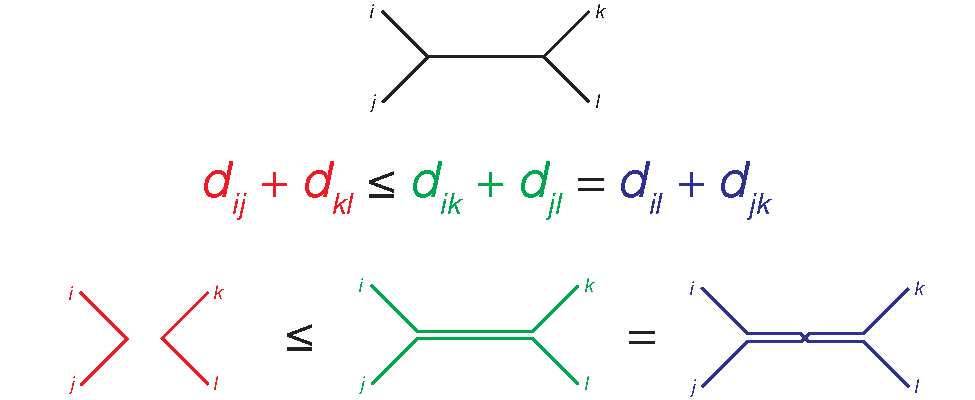
\includegraphics[]{./fig/background/four_point_condition.pdf}
\caption[The four point condition for additivity]{A visual interpretation of the four point condition for additivity. For any four leaves, there exists a labeling $\{i,j,k,l\}$ such that $d_{ij}+d_{kl}\leq d_{ik}+d_{il} = d_{il}+d_{jk}$. Of the three possible ways of arranging the sums of distances, two will involve traversing the internal branch, while one will involve only external branches.}
\label{background:fig:four_point_condition}
\end{figure}

Given that we can associate a distance matrix to se
Only in the case of perfectly additive data will a tree be able to exactly fit the matrix.
\kje{(Define additivity -- four point condition.)}

Sequence data can fail to be additive for several reasons.
First, sequencing error.
Errors can introduce noise into the measured genetic distances.
Second, homoplasy.
A homoplasy occurs when the same mutation is introduced multiple times in a set of organisms.
The presence of homoplasy will underestimate genetic distance between taxa.
Third, reticulate evolution.
As described previously, in cases of reticulate evolution no tree will accurately describe the observed data.

\subsubsection{Number of Tree Topologies}

The number of unrooted bifurcating tree topologies with $L$ leaves is $(2L-5)!!$.\footnote{The double factorial is defined as $n!!=n(n-2)(n-4)\cdots$.}
This can be easily shown using induction.
For $L=3$, we have $\mathcal{T}(3)=1$ and $3$ branches.
To pass to $L=4$, we can add the fourth leaf to any of the $3$ branches, resulting in $3$ different topologies.
For $L=4$, we have $\mathcal{T}(4)=3$.
Every time we add a leaf, we add two branches -- one external and one internal.
For $L=n$, we have $\mathcal{T}(n)=(2n-5)!!$ and $2n-3$ branches.
For $L=n+1$, we can add the new external branch to any of the current $2n-3$ branches.
A rooted tree with $L$ leaves can be considered as an unrooted tree with $L+1$ leaves.
Therefore, the number of rooted bifurcating tree topologies with $L$ leaves is $(2L-3)!!$
As can be seen, the number of tree topologies explodes with the number of leaves.
Fitch quote: \emph{more than 20 species, more than Avogadro's number of topologies.}

\subsubsection{Space of Phylogenetic Trees}

** Needs work.

A phylogenetic tree is characterized by its number of leaves, the particular tree topology, and the length of each branch.
Tree space refers to an abstract construction that represents each possible tree as a point in a geometric space.
Abstract studies of tree space were initiated by Billera, Holmes, and Vogtmann (BHV) in \cite{Billera:2001tv}.

In the BHV model, each point represents an unrooted binary tree with $L$ leaves and strictly positive branch lengths.

Number of interior edges $r=L-3$, a particular additive tree can be plotted as a point in the positive open orthant $(0,\infty)^{r}$.

A single orthant corresponds to a single tree topology.

\begin{figure}
\centering
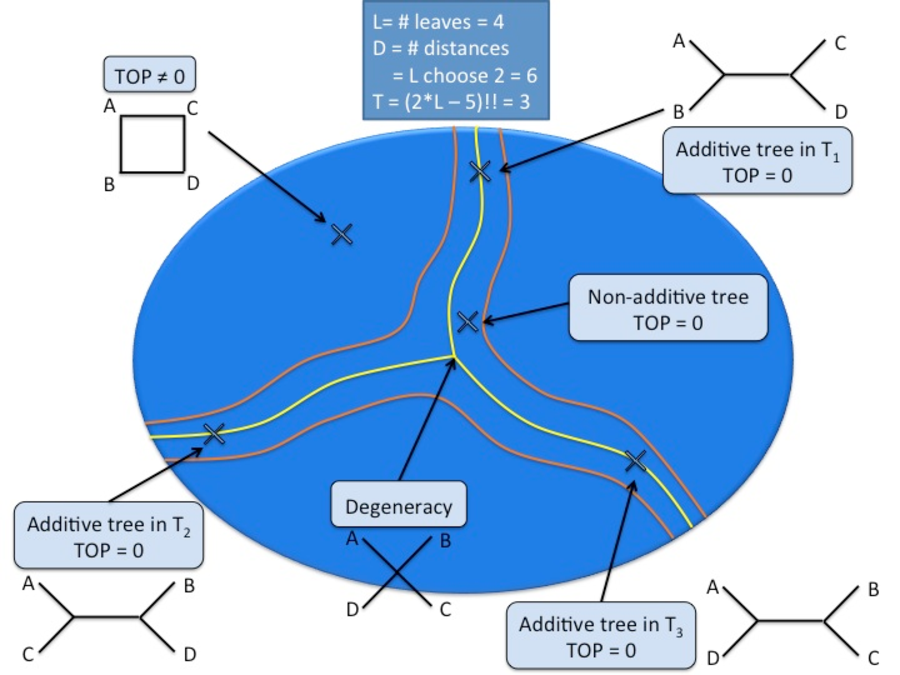
\includegraphics[]{./fig/TreeSpace.pdf}
\caption{Tree Space}
\label{background:fig:TreeSpace}
\end{figure}

\subsubsection{Phylogenetic Networks}

There are several existing methods for representing reticulate evolution.
Most of these methods generalize phylogenetic trees into \emph{phylogenetic networks}, which attempt to reconcile the presence of horizontal evolution in sequence data.
However, most simply present corrections to phylogenetic trees, which can fail in cases where horizontal evolution is pervasive, as in many prokaryote datasets.
Additionally, the resulting neteworks can be complex and difficult to interpret quantitatively.
\kje{[Expand. See Morrison review. Split Networks.]}

